\chapter{\IfLanguageName{dutch}{Stand van zaken}{State of the art}}%
\label{ch:stand-van-zaken}

% Tip: Begin elk hoofdstuk met een paragraaf inleiding die beschrijft hoe
% dit hoofdstuk past binnen het geheel van de bachelorproef. Geef in het
% bijzonder aan wat de link is met het vorige en volgende hoofdstuk.

% Pas na deze inleidende paragraaf komt de eerste sectiehoofding.
\
\section{Auth technologieën}%
\label{sec:auth-technologieën}
In eerste instantie wordt bekeken welke huidge technologieën er vandaag de dag bestaan en welke de meest gebruikte zijn. Dit omdat er eerst een goede kennis
moet worden gelegd van de huidige technologieën vooraleer er kan worden overgegaan naar de volgende stappen.


\subsection{OAuth 2.0}%
\label{subsec:oauth-2.0}
\autocite{Hardt2012}
OAuth 2.0 wordt gebruikt om toegang tot bronnen te delegeren zonder gebruikersreferenties te delen. Het is een autorisatie framework en wordt dus niet gebruikt voor het authenticeren van gebruikers. Vaak gebruikt om Single Sign On (SSO) en toegangsdelegatie in te schakelen. Kan worden gebruikt in web- en mobiele applicaties en ondersteunt verschillende authenticatiemechanismen.
Dit moet worden geïmplementeerd omdat de service een API gaat aanbieden die toegankelijk is voor applicaties van derden en dus wordt gebruikt voor authentificatie.

\subsubsection{Access Tokens}%
\label{subsubsec:access-tokens}
Access Tokens zijn inloggegevens die worden gebruikt om toegang te krijgen tot bronnen. Access Tokens worden door de autorisatieserver aan de client uitgegeven en worden door de client gebruikt om toegang te krijgen tot bronnen die worden beschermd door de autorisatieserver. Access Tokens zijn bedoeld voor gebruik met bronservers en worden nooit naar autorisatieservers verzonden.

\subsubsection{Refresh Tokens}%
\label{subsubsec:refresh-tokens}
Refresh Tokens zijn inloggegevens die worden gebruikt om Access Tokens te verkrijgen. Refresh Tokens worden door de autorisatieserver aan de client uitgegeven en worden gebruikt om een nieuw Access Tokens te verkrijgen wanneer het huidige Access Token ongeldig wordt of verloopt, of om extra Access Tokens met een identiek of beperkter bereik te verkrijgen. Het uitgeven van een Refresh Tokens is optioneel, ter beoordeling van de autorisatieserver. Als de autorisatieserver een Refresh Token afgeeft, wordt deze meegenomen bij de uitgifte van een Access Token. In tegenstelling tot Access Tokens zijn Refresh Tokens alleen bedoeld voor gebruik met autorisatieservers en worden ze nooit naar bronservers verzonden.
Dit zou kunnen worden geïmplementeerd met een kortere vervaldatum van het Access Token in plaats van een Access Token met een zeer lange vervaldatum, maar toch de black list met Access Tokens gebruiken.
\begin{figure}[h]
  \centering
  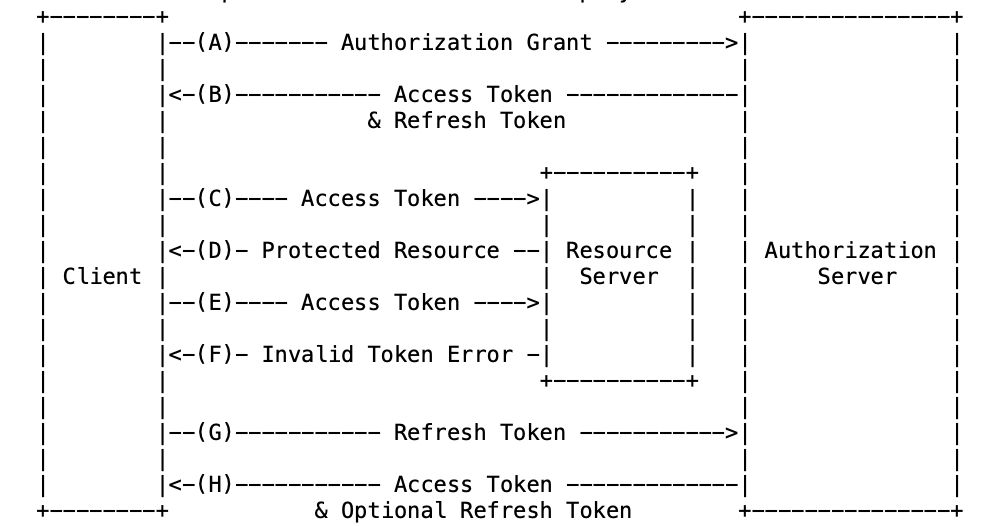
\includegraphics[width=0.5\textwidth]{oauth2.png}
  \caption{OAuth 2.0 verloop}
  \label{fig:example1}
\end{figure}

\subsubsection{Client Types}%
\label{subsubsec:client-types}
Er zijn twee soorten clients die OAuth 2.0 kunnen gebruiken:
\begin{enumerate}[label=\textbf{-}]
    \item Confidential Clients: \\
    Een client die in staat is om de clientgeheimen te beschermen en te vertrouwen op de autorisatieserver om de identiteit van de client te verifiëren. Dit type client is in staat om zowel de autorisatiecode als de Access Token te ontvangen. (bijvoorbeeld een client geïmplementeerd op een beveiligde server met beperkte toegang tot de clientgegevens)
  
    \item Public Clients: \\
    Een client die niet in staat is om de clientgeheimen te beschermen en daarom niet in staat is om de identiteit van de client te verifiëren. Dit type client is alleen in staat om de Access Token te ontvangen. (bijvoorbeeld clients die worden uitgevoerd op het apparaat dat wordt gebruikt door de eigenaar van de bron, zoals een geïnstalleerde native applicatie of een webbrowsergebaseerde applicatie)
\end{enumerate}
Hier zijn enkele applicaties met hun respectievelijke clienttypes:
\begin{enumerate}[label=\textbf{-}]
    \item Web applicatie: \\
    Een webapplicatie die wordt uitgevoerd op een webserver. Dit type client is een confidential client. De clientgeheimen alsook de Access Token worden opgeslagen op de webserver en zijn niet toegankelijk voor de resource-eigenaar.
  
    \item User-Agent gebaseerde applicatie: \\
    Een applicatie die wordt uitgevoerd in de user-agent van de resource-eigenaar, zoals een webbrowser. Dit type client is een public client. De clientgeheimen zijn toegankelijk voor de resource-eigenaar en kunnen niet worden beschermd tegen ongeautoriseerde toegang.
  
    \item Native applicatie: \\
    Een applicatie die wordt uitgevoerd op het apparaat dat wordt gebruikt door de resource-eigenaar, zoals een desktopapplicatie of een mobiele applicatie. Dit type client is een public client. De clientgeheimen zijn toegankelijk voor de resource-eigenaar en kunnen niet worden beschermd tegen ongeautoriseerde toegang.
\end{enumerate}


\subsubsection{Client Authentication}
\label{subsubsec:client-authentication}
De client moet bij elk verzoek niet meer dan één authenticatiemethode gebruiken.

\subsubsection{Endpoints}%
\label{subsubsec:endpoints}
\begin{enumerate}[label=\textbf{-}]
    \item Authorization Endpoint: \\
    Dit endpoint wordt door de clienttoepassing gebruikt om autorisatie van de resource-eigenaar te verkrijgen. Meestal houdt dit in dat de gebruiker wordt omgeleid naar het autorisatie-endpoint van de autorisatieserver, waar hij/zij kan inloggen en machtigingen kan verlenen aan de clienttoepassing. Na het verlenen van autorisatie leidt de autorisatieserver de gebruiker terug naar de clienttoepassing met een autorisatiecode of Access Token.
    \newline
    Een response_type van "code" geeft aan dat de clienttoepassing een autorisatiecode wil ontvangen. Een response_type van "token" geeft aan dat de clienttoepassing een Access Token wil ontvangen.
  
    \item Token Endpoint: \\
    Na het verkrijgen van autorisatie van de eigenaar van de bron, wisselt de clienttoepassing de autorisatiecode uit voor een Access Token door een verzoek naar het token endpoint te sturen. Dit endpoint is verantwoordelijk voor het authenticeren van de client en het uitwisselen van de autorisatiecode voor een Access Token. Het token endpoint wordt door de client gebruikt om een Access Token te verkrijgen door de Authorization Grant of Refresh Token te presenteren.
    \newline
    Met andere woorden is dit endpoint optioneel, omdat de autorisatieserver de Access Token ook kan retourneren in de respons van het autorisatieverzoek. In dit geval is het token endpoint niet nodig.
    \newline
    Men kan dit endpoint ook gebruiken om een nieuwe Access Token te verkrijgen met behulp van een Refresh Token. Dit is handig wanneer de Access Token verloopt of ongeldig wordt.
  
    \item Redirection Endpoint: \\
    Dit is niet bepaald een endpoint, maar het is een cruciaal onderdeel van de OAuth-stroom. Het is de URI waar de autorisatieserver de user-agent (meestal een webbrowser) omleidt nadat de resource-eigenaar toegang tot de clienttoepassing heeft verleend/geweigerd. De redirect-URI bevat doorgaans parameters zoals de autorisatiecode of het Access Token. Wanneer een redirect-URI is opgenomen in een autorisatieverzoek, moet de autorisatieserver de ontvangen waarde vergelijken en matchen met ten minste één van de geregistreerde redirect-URI's (of URI-componenten), als er redirect-URI's zijn geregistreerd. Als de clientregistratie de volledige redirect-URI bevatte, moet de autorisatieserver de twee URI's vergelijken met behulp van eenvoudige string vergelijking. Als de validatie van een autorisatieverzoek mislukt vanwege een ontbrekende, ongeldige of niet-overeenkomende redirect-URI, moet de autorisatieserver de eigenaar van de bron op de hoogte stellen van de fout en moet de user-agent niet automatisch worden omgeleid naar de ongeldige redirect-URI.
  \end{enumerate}

\subsubsection{Authorization request}%
\label{subsubsec:authorization-request}
De client maakt een verzoek naar de autorisatieserver om autorisatie te verkrijgen. Het verzoek bevat de volgende parameters:
\begin{enumerate}[label=\textbf{-}]
    \item response type: \\
    Deze parameter geeft het gewenste responstype aan. De waarde moet "code" zijn voor autorisatiecode of "token" voor Access Token.
  
    \item client id: \\
    Deze parameter geeft de client-ID van de clienttoepassing aan. De waarde moet overeenkomen met de geregistreerde client-ID van de clienttoepassing.
  
    \item redirect uri: \\
    Deze parameter geeft de URI aan waar de autorisatieserver de gebruiker na autorisatie moet omleiden. De waarde moet overeenkomen met een van de geregistreerde redirect-URI's van de clienttoepassing.
  
    \item scope: \\
    Deze parameter geeft de machtigingen aan die de clienttoepassing wil verkrijgen. De waarde moet een spatiegescheiden lijst van machtigingen zijn.
  
    \item state: \\
    Deze parameter geeft een willekeurige, niet-voorspelbare waarde aan die door de clienttoepassing wordt gegenereerd. De waarde moet worden gebruikt om CSRF-aanvallen te voorkomen.
  \end{enumerate}
  En kan er als volgt uitzien:
  \begin{verbatim}
    GET /authorize?response_type=code&client_id=s6BhdRkqt3&
    state=xyz&redirect_uri=https%3A%2F%2Fclient%2Eexample%2Ecom%2Fcb
    HTTP/1.1
    Host: server.example.com
  \end{verbatim}
    

\subsubsection{Authorization reponse}%
\label{subsubsec:authorization-reponse}
De autorisatieserver verleent autorisatie aan de clienttoepassing en leidt de gebruiker terug naar de clienttoepassing met een autorisatiecode of Access Token. Het antwoord bevat de volgende parameters:
\begin{enumerate}[label=\textbf{-}]
    \item code: \\
    Deze parameter geeft de autorisatiecode aan die door de autorisatieserver is gegenereerd. De autorisatiecode wordt gebruikt door de clienttoepassing om een Access Token te verkrijgen.
  
    \item state: \\
    Deze parameter geeft de waarde van de state-parameter van het autorisatieverzoek aan. De waarde moet overeenkomen met de waarde die door de clienttoepassing is verstrekt.
  \end{enumerate}
  En kan er als volgt uitzien:
  \begin{verbatim}
    HTTP/1.1 302 Found
    Location: https://client.example.com/cb?code=SplxlOBeZQQYbYS6WxSbIA&state=xyz
  \end{verbatim}

\subsubsection{Error response}%
\label{subsubsec:error-response}
Als het verzoek mislukt vanwege een ontbrekende, ongeldige of niet-overeenkomende redirect-URI, of als de client-ID ontbreekt of ongeldig is, moet de autorisatieserver de eigenaar van de bron op de hoogte stellen van de fout en moet de user-agent niet automatisch omleiden naar de ongeldige redirect-URI.

\subsubsection{Een Access Token vernieuwen}%
\label{subsubsec:een-access-token-vernieuwen}
Als de autorisatieserver een Refresh Token aan de client heeft uitgegeven, doet de cliënt een vernieuwingsverzoek aan het token endpoint.
Indien geldig en geautoriseerd, geeft de autorisatieserver een Access Token uit. Als de verificatie van het verzoek is mislukt of ongeldig is, retourneert de autorisatieserver een foutreactie.
De autorisatieserver kan een nieuw Refresh Token uitgeven, in welk geval de cliënt het oude Refresh Token moet weggooien en vervangen door het nieuwe Refresh Token. De autorisatieserver kan het oude Refresh Token intrekken nadat een nieuw Refresh Token aan de client is uitgegeven. Als er een nieuw Refresh Token wordt uitgegeven, moet het bereik van het Refresh Token identiek zijn aan dat van het Refresh Token dat door de client in de aanvraag is opgenomen.

\subsubsection{Beveiligingsoverwegingen}
\label{subsubsec:beveiligingsoverwegingen}
\begin{enumerate}[label=\textbf{-}]
    \item Client Impersonation: \\
    Een kwaadwillende client kan zich voordoen als een andere client en toegang krijgen tot beschermde bronnen als de nagebootste client er niet in slaagt of niet in staat is zijn clientreferenties vertrouwelijk te houden.

    \item Access Tokens: \\
    De autorisatieserver moet ervoor zorgen dat Access Tokens niet door onbevoegde partijen kunnen worden gegenereerd, gewijzigd of geraden om geldige Access Tokens te produceren.

    \item Refresh Tokens: \\
    De autorisatieserver moet de binding tussen het Refresh Token en de clientidentiteit verifiëren wanneer de clientidentiteit kan worden geverifieerd. Wanneer clientauthenticatie niet mogelijk is, moet de autorisatieserver andere middelen inzetten om misbruik van Refresh Token te detecteren. De autorisatieserver zou bijvoorbeeld Refresh Token rotatie kunnen gebruiken, waarbij een nieuw Refresh Token wordt uitgegeven bij elke vernieuwingsreactie van het Access Token. Het vorige Refresh Token wordt ongeldig gemaakt, maar behouden door de autorisatieserver. Als een Refresh Token wordt aangetast en vervolgens door zowel de aanvaller als de legitieme client wordt gebruikt, zal een van hen een ongeldig Refresh Token presenteren, dat de autorisatieserver op de hoogte stelt van de inbreuk. De autorisatieserver moet ervoor zorgen dat Refresh Tokens niet door onbevoegde partijen kunnen worden gegenereerd, gewijzigd of geraden dat ze geldige Refresh Tokens produceren.

    \item Request Confidentiality: \\
    Access Tokens, Refresh Tokens, wachtwoorden voor resource-eigenaren en klantreferenties moeten niet openbaar worden verzonden. De parameters "state" en "scope" moeten geen gevoelige klant- of resource-eigenaarinformatie in platte tekst bevatten, omdat deze via onveilige kanalen kunnen worden verzonden of onveilig kunnen worden opgeslagen.
\end{enumerate}


\subsection{OAuth 2.0 voor Native Apps}%
\label{subsec:oauth-2.0-voor-native-apps}
\autocite{Denniss2017}
Een native app is een app die door de gebruiker op zijn apparaat wordt geïnstalleerd, in tegenstelling tot een webapp die alleen in de browsercontext wordt uitgevoerd. Apps die zijn geïmplementeerd met behulp van webgebaseerde technologie maar worden gedistribueerd als een native app, de zogenaamde "hybride apps", worden voor het doel van deze specificatie beschouwd als gelijkwaardig aan native apps.
OAuth 2.0-autorisatieverzoeken van native apps worden het best, en het liefst alleen, gedaan via externe user-agents, voornamelijk de browser van de gebruiker. Het andere alternatief is het gebruik van ingebedde user-agents. Deze aanpak heeft veel nadelen, waaronder het feit dat de host-app gebruikersgegevens en cookies kan kopiëren en dat de gebruiker zich in elke app helemaal opnieuw moet authenticeren. Autorisatieverzoeken voor native apps die de browser gebruiken, zijn veiliger en kunnen profiteren van de authenticatiestatus van de gebruiker. Door de bestaande authenticatiesessie in de browser te kunnen gebruiken, is eenmalige aanmelding (SSO) mogelijk, omdat gebruikers zich niet telkens opnieuw hoeven te authenticeren bij de autorisatieserver wanneer ze een nieuwe app gebruiken.
Om deze best practices te ondersteunen, dienen bepaalde OAuth-serverimplementaties die vertrouwen op alle clients als vertrouwelijk (confidential) voor het web, openbare (public) native app-clients en hun bijbehorende soorten redirect-URI's te erkennen.
\begin{figure}[h]
  \centering
  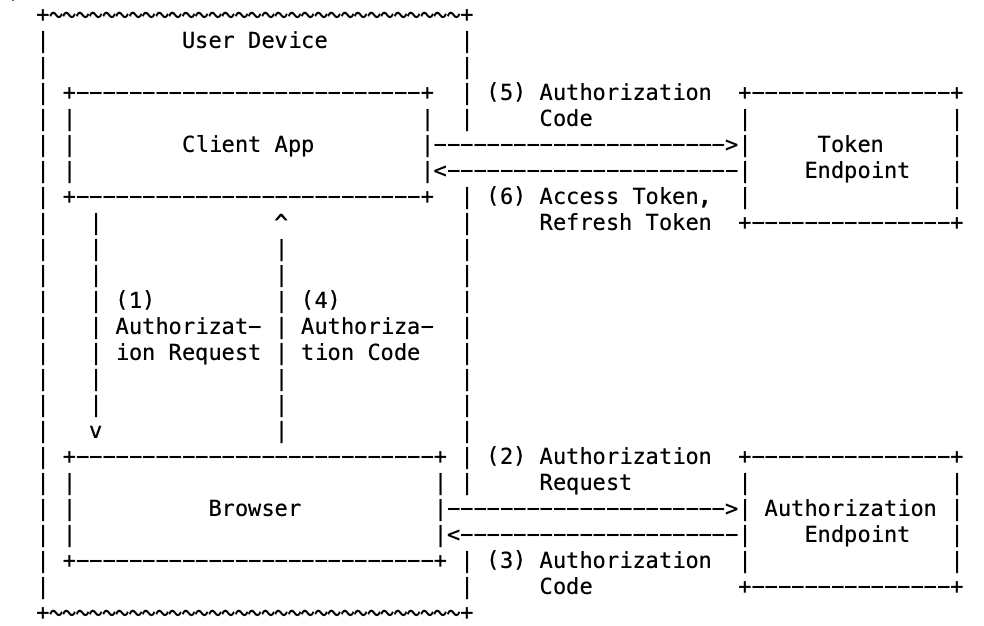
\includegraphics[width=0.5\textwidth]{oauth2_native.png}
  \caption{OAuth 2.0 verloop in native apps}
  \label{fig:example2}
\end{figure}
\newline
Dit wordt bereikt door het autorisatieverzoek in de browser te openen en een redirect-URI te gebruiken die het autorisatieantwoord terugstuurt naar de native app.
\newline
\newline
Het ontvangen van de Autorisatiereactie in een Native App gebeurt ook via een redirect URI, er zijn verschillende opties:
\newline
- Omleiding van URI-schema voor privégebruik: nadat de auth-server het verzoek heeft voltooid, wordt deze omgeleid naar de omleidings-URI van de client, com.example.app:/oauth2redirect/example-provider, dit resulteert erin dat het besturingssysteem de native app start en de URI als startparameter.
\newline
- Geclaimde 'https'-schema-URI-omleiding: https://app.example.com/oauth2redirect/example-provider, door de app geclaimde 'https'-schema-omleidings-URI's hebben enkele voordelen vergeleken met andere native app-omleidingsopties, omdat de identiteit van de de bestemmingsapp wordt door het besturingssysteem gegarandeerd aan de autorisatieserver. Om deze reden moeten native apps deze waar mogelijk boven de andere opties gebruiken.
\newline
- Loopback Interface Redirection: http://127.0.0.1:51004/oauth2redirect/example-provider, voornamelijk voor desktop-apps die een poort op de loopback-netwerkinterface kunnen openen zonder speciale machtigingen nodig te hebben, kunnen de loopback-interface gebruiken om de OAuth te ontvangen omleiden.


\subsection{OAuth 2.0: Bearer Token gebruik}%
\label{subsec:oauth-2.0-bearer-token-gebruik}
OAuth 2.0 bearer tokens kunnen worden gebruikt in HTTP-verzoeken om toegang te krijgen tot beveiligde bronnen \autocite[p.~{Section 1.0}]{Jones2012}.
Een bearer token is een token dat kan worden gebruikt door iedereen die eigenaar is van het token, zonder dat er bewijs nodig is van het bezit van cryptografisch materiaal \autocite[p.~{Section 1.2}]{Jones2012}.
Er worden drie manieren beschreven om een bearer token in een aanvraag op te nemen: in de Authorization-header, als een formuliergecodeerde body-parameter of als een URI-queryparameter \autocite[p.~{Section 2.1}]{Jones2012}. Als een verzoek mislukt, moet de bronserver een 401-statuscode en een foutcode retourneren, zoals 'invalid\verb|_|request', 'invalid\verb|_|token' of 'insufficient\verb|_|scope' \autocite[p.~{Section 3.0}]{Jones2012}.
Het gebruik van TLS, het valideren van certificaten, het uitgeven van tokens voor de korte termijn en het niet opslaan van tokens in cookies zijn elk sterk aanbevolen \autocite[p.~{Section 5.0}]{Jones2012}.


\subsection{JWT huidige Best Practices}%
\label{subsec:jwt-huidige-best-practices}
Deze sectie lijst de bekende en mogelijke problemen op met JWT-implementaties en -inzet. Elk probleem wordt gevolgd door verwijzingen naar een of meer maatregelen om deze problemen te verhelpen.
\begin{enumerate}[label=\textbf{-}]
    \item Zwakke Handtekeningen en Onvoldoende Validatie van Handtekeningen
    \item Zwakke Symmetrische Sleutels: Deze zijn even onveilig als makkelijk te onthouden wachtwoorden.
    \item Onjuiste Samenstelling van Encryptie en Handtekening: Sommige bibliotheken die een JWE-versleutelde JWT ontcijferen om een JWS-ondertekend object te verkrijgen, valideren niet altijd de interne handtekening.
    \item Plaintext lek door Analyse van Cijfertekstlengte: Veel encryptiealgoritmen lekken informatie over de lengte van de oorspronkelijke tekst.
    \item Onveilig Gebruik van Elliptische Curve-Encryptie
    \item Veelvoud van JSON-coderingen
    \item Substitutieaanvallen: Dit zijn aanvallen waarbij een ontvanger een JWT krijgt die voor hem bedoeld was en probeert deze te gebruiken bij een andere ontvanger waarvoor die JWT niet bedoeld was.
    \item Kruis-JWT-verwarring: Gevallen voorkomen waarin JWT-tokens die zijn uitgegeven voor een bepaald doel, worden ondermijnd en gebruikt voor een ander doel.
    \item Indirecte Aanvallen op de Server
\end{enumerate}
Best Practices
\begin{enumerate}[label=\textbf{-}]
  \item Voer algoritmeverificatie uit: Zorg ervoor dat de algoritmen die worden gebruikt voor het ondertekenen en versleutelen van JWT's veilig zijn.
  \item Gebruik geschikte algoritmen: Gebruik veilige algoritmen voor het ondertekenen en versleutelen van JWT's.
  \item Valideer alle cryptografische bewerkingen: Zorg ervoor dat alle cryptografische bewerkingen correct worden uitgevoerd.
  \item Valideer cryptografische invoer: Zorg ervoor dat alle invoer voor cryptografische bewerkingen correct is. Dit omvat het valideren van de lengte van de invoer, het controleren van de invoer op ongeldige tekens en het valideren van de invoer tegen een lijst met bekende sleutels.
  \item Zorg ervoor dat cryptografische sleutels voldoende entropie hebben: Entropie is een maat voor de onvoorspelbaarheid van een reeks gegevens.
  \item Vermijd compressie van coderingsinvoer: Compressie van coderingsinvoer kan leiden tot lekken van informatie over de oorspronkelijke tekst.
  \item Gebruik UTF-8: Zorg ervoor dat alle tekst die wordt gebruikt in JWT's wordt gecodeerd in UTF-8.
  \item Valideer de uitgever en het onderwerp: Issuer en Subject
  \item Gebruik en valideer doelgroep: Audience
  \item Vertrouw ontvangen claims niet
  \item Gebruik expliciet typen
  \item Gebruik wederzijds exclusieve validatieregels voor verschillende soorten JWT's
\end{enumerate}
\autocite{Sheffer2020}


\subsection{OpenID Connect}%
\label{subsec:openid-connect}
OpenID Connect is een identiteitslaag bovenop OAuth 2.0, dat wordt gebruikt voor authenticatie. Het is een eenvoudige identiteitslaag die bovenop OAuth 2.0 is gebouwd en die de authenticatie van gebruikers mogelijk maakt. OpenID Connect biedt een eenvoudige manier om gebruikers te verifiëren en toegang te verlenen tot applicaties en services. Het maakt gebruik van JSON Web Tokens (JWT's) om claims over gebruikers te verstrekken en om gebruikers te verifiëren. OpenID Connect is ontworpen om eenvoudig te implementeren en te gebruiken en biedt een veilige en betrouwbare manier om gebruikers te verifiëren en toegang te verlenen tot applicaties en services.
\newline
\newline
OpenID Connect biedt een aantal voordelen ten opzichte van traditionele authenticatiemethoden, waaronder:
\begin{enumerate}[label=\textbf{-}]
    \item Eenvoudige implementatie: OpenID Connect is eenvoudig te implementeren en te gebruiken en biedt een gestandaardiseerde manier om gebruikers te verifiëren en toegang te verlenen tot applicaties en services.
    \item Veilige en betrouwbare authenticatie: OpenID Connect maakt gebruik van JSON Web Tokens (JWT's) om claims over gebruikers te verstrekken en om gebruikers te verifiëren. Dit biedt een veilige en betrouwbare manier om gebruikers te verifiëren en toegang te verlenen tot applicaties en services.
    \item Flexibiliteit: OpenID Connect biedt een flexibele manier om gebruikers te verifiëren en toegang te verlenen tot applicaties en services. Het ondersteunt verschillende authenticatiemethoden en kan worden gebruikt in een breed scala van toepassingen.
    \item Schaalbaarheid: OpenID Connect is schaalbaar en kan worden gebruikt in grote en complexe omgevingen. Het biedt een betrouwbare manier om gebruikers te verifiëren en toegang te verlenen tot applicaties en services.
\end{enumerate}
\autocite{Sakimura2014}


\subsection{Biometrische authenticatie}%
\label{subsec:biometrische-authenticatie}
Biometrische authenticatie is een methode voor het verifiëren van de identiteit van een persoon op basis van fysieke of gedragskenmerken. Het maakt gebruik van biometrische gegevens zoals vingerafdrukken, gezichtsherkenning en irisscans om gebruikers te verifiëren en toegang te verlenen tot systemen, applicaties en gegevens. Biometrische authenticatie biedt een veilige en gebruiksvriendelijke manier om gebruikers te verifiëren en biedt bescherming tegen identiteitsdiefstal en fraude. Het wordt gebruikt in een breed scala van toepassingen, waaronder mobiele apparaten, computers, toegangscontrolesystemen en financiële transacties. Biometrische authenticatie wordt steeds populairder vanwege de groeiende behoefte aan veilige en gemakkelijke manieren om gebruikers te verifiëren en hun identiteit te beschermen. Het biedt een effectieve manier om de beveiliging van systemen en gegevens te verbeteren en biedt een betere gebruikerservaring dan traditionele wachtwoordgebaseerde methoden. Biometrische authenticatie wordt beschouwd als een van de meest veilige en betrouwbare methoden voor het verifiëren van de identiteit van een persoon en wordt steeds vaker gebruikt in verschillende sectoren, waaronder banksector, gezondheidszorg, overheid en bedrijfsleven.
\newline
\newline
Misbruik van traditionele beveiligings maatregelen, zoals wachtwoorden, heeft geleid tot de ontwikkeling van biometrische authenticatie als een veiligere en betrouwbaardere methode voor het verifiëren van de identiteit van een persoon. Biometrische gegevens zijn uniek voor elke persoon en kunnen niet, in het slechtste geval moeilijk, worden nagemaakt of gestolen, waardoor ze een effectieve manier zijn om de identiteit van een persoon te verifiëren.

\subsubsection{Gezichtsherkenning}%
\label{subsubsec:gezichtsherkenning}
Deze systemen gebruiken de unieke gelaatstrekken van een persoon om deze te identificeren. Het wordt op verschillende plaatsen gebruikt, zoals op smartphones, creditcardbetalingen en bij wetshandhaving.

\subsubsection{Vingerafdrukherkenning}%
\label{subsubsec:vingerafdrukherkenning}
Vingerafdrukauthenticatie maakt gebruik van de unieke vingerafdruk van een persoon om zijn identiteit te verifiëren. Het kan worden gebruikt om alles te beveiligen, van mobiele apparaten tot auto's en zelfs gebouwen, waardoor het de meest wijd verspreide biometrische authenticatietechnologie is.

\subsubsection{Oogherkenning}%
\label{subsubsec:oogherkenning}
Oogherkenning maakt gebruik van het unieke patroon van iemands iris of netvlies om iemand te identificeren. Omdat dit type biometrische authenticatie moeilijker te implementeren is, komt het minder vaak voor dan de andere soorten biometrische authenticatieopties. Een irisscan vereist een infraroodlichtbron, een camera die IR kan zien en minimale lichtvervuiling om nauwkeurigheid te garanderen. Hoewel het uitdagingen met zich meebrengt, is het een van de meest nauwkeurige biometrische authenticatiesystemen die beschikbaar zijn als aan deze voorwaarden wordt voldaan. Oogherkenning wordt over het algemeen gebruikt in situaties waarin de veiligheid het meest kritisch is, zoals bij nucleaire onderzoeksfaciliteiten, enz.

\subsubsection{Spraakherkenning}%
\label{subsubsec:spraakherkenning}
Spraakherkenning maakt gebruik van de toon, toonhoogte en frequenties die uniek zijn voor een individu om deze te authenticeren. Dit is de meest gebruikte biometrie om gebruikers te verifiëren wanneer ze contact opnemen met een callcenter voor klantenservice (bijvoorbeeld online bankieren).

\subsubsection{Gangherkenning}%
\label{subsubsec:gangherkenning}
Gangherkenning authenticeert door gebruik te maken van de manier waarop iemand loopt om hem/haar te identificeren. Elke persoon loopt een beetje anders, dus de manier waarop iemand de ene voet voor de andere zet, is een effectieve manier om zijn identiteit te verifiëren. Op dit moment is het geen gebruikelijke vorm van authenticatie, maar de verwachting is dat dit steeds gebruikelijker zal worden naarmate toekomstige vormen van authenticatie populairder worden.

\subsubsection{Aderherkenning}%
\label{subsubsec:aderherkenning}
Bij aderherkenning wordt gebruik gemaakt van het patroon van de bloedvaten in de hand of vinger van een persoon om deze te identificeren. Bij dit type biometrische authenticatie wordt gebruik gemaakt van infraroodlicht om de aderen onder de huid van uw handen of vingers in kaart te brengen. Aderherkenning is uiterst nauwkeurig, meer dan netvlies-/irisherkenning.

\subsubsection{Multimodale biometrische authenticatie}%
\label{subsubsec:multimodale-biometrische-authenticatie}
Eerst moeten we begrijpen wat een unimodaal biometrisch authenticatie systeem is. Dit is een systeem dat verifieert op basis van 1 biometrische methode, het is dan uiteraard niet verwondelijk dat dit soort systemen heel kwetsbaar zijn voor spoofing.
\newline
\newline
Dit is waar multimodale biometrische authenticatie in beeld komt. Het is een aanpak waarin meerdere biometrische eigenschappen worden gebruikt om de identiteit van een persoon te verifiëren. Dit kan bijvoorbeeld een combinatie zijn van gezichtsherkenning en vingerafdrukherkenning. Door meerdere biometrische eigenschappen te combineren, wordt de nauwkeurigheid van het authenticatiesysteem verhoogd en wordt het moeilijker voor aanvallers om het systeem te misleiden. Multimodale biometrische authenticatie wordt steeds populairder vanwege de groeiende behoefte aan veilige en betrouwbare authenticatiesystemen.

\subsubsection{De voordelen van biometrische authenticatie}%
\label{subsubsec:de-voordelen-van-biometrische-authenticatie}
\begin{enumerate}[label=\textbf{-}]
  \item Identiteitsverzekering: \\
  Biometrische identificatie biedt de antwoorden op “iets wat een persoon heeft en is” en helpt de identiteit te verifiëren. Biometrische authenticatie zorgt voor meer zekerheid voor eindgebruikers. De geavanceerde software laat providers weten dat een persoon is wie ze beweren te zijn door middel van een tastbare, reële eigenschap. Zelfs als een cyberaanvaller het wachtwoord van een gebruiker of het antwoord op zijn beveiligingsvraag kent, is het onmogelijk dat hij of zij een vingerafdruk of irisscan kan dupliceren.

  \item Gebruiksgemak: \\
  Hoewel biometrische authenticatie meer technisch van aard is met betrekking tot het interne proces, is het over het algemeen gemakkelijk en snel vanuit het oogpunt van de gebruiker. Door een vingerafdrukscanner te gebruiken om een account te ontgrendelen of gezichtsherkenning, vermindert u het aantal keren dat u moet inloggen met een lang wachtwoord dat meerdere speciale tekens bevat die u waarschijnlijk uiteindelijk zult vergeten.

  \item Fraudedetectie: \\
  Biometrie is bijna onmogelijk te repliceren. Ze zijn moeilijk te repliceren en te stelen, en de kans is slechts ongeveer 1 op 64 miljard \autocite{Baker2021} \autocite{Lee2013} dat jouw vingerafdruk precies overeenkomt met die van iemand anders. Het is zeer onwaarschijnlijk dat een hacker toegang krijgt tot alles dat met biometrie is beveiligd.
\end{enumerate}

\subsubsection{De nadelen van biometrische authenticatie}%
\label{subsubsec:de-nadelen-van-biometrische-authenticatie}
\begin{enumerate}[label=\textbf{-}]
  \item Hackbaar: \\
  Biometrie kan nog steeds worden gehackt. Bedrijven en overheden die de persoonlijke gegevens van gebruikers verzamelen en opslaan, worden voortdurend bedreigd door hackers. Als ze echter het slachtoffer worden van een datalek, zijn biometrische gegevens onvervangbaar en moeten organisaties zorgvuldig omgaan met de biometrische gegevens van gebruikers.

  \item Gedeeltelijke overeenkomsten: \\
  De meeste gangbare biometrische authenticatiemethoden zijn afhankelijk van gedeeltelijke informatie om de identiteit van een gebruiker te verifiëren. Tijdens het registratieproces voor het registreren van uw vingerafdruk worden bijvoorbeeld gegevens van uw gehele afdruk gebruikt en omgezet in gegevens. Tijdens toekomstige authenticatie zijn echter slechts gedeeltelijke vingerafdrukgegevens nodig om uw identiteit te verifiëren, zodat het steeds sneller gaat.

  \item Onnauwkeurigheid: \\
  Biometrische authenticatie is niet perfect en kan fouten maken bij het identificeren van gebruikers. Dit kan leiden tot frustratie bij gebruikers en kan de veiligheid van het systeem in gevaar brengen. Het is belangrijk om de nauwkeurigheid van biometrische authenticatie te evalueren voordat u het implementeert.
\end{enumerate}


\subsection{WebAuthn}%
\label{subsec:webauthn}
WebAuthn is een W3C-specificatie die een webstandaard biedt voor biometrische authenticatie. Het is bedoeld om een veilige en gebruiksvriendelijke manier te bieden om gebruikers te verifiëren zonder dat ze wachtwoorden hoeven te onthouden. WebAuthn maakt gebruik van openbare en privésleutels om gebruikers te verifiëren en biedt een veilige manier om in te loggen op websites en applicaties. Het maakt gebruik van biometrische gegevens zoals vingerafdrukken, gezichtsherkenning en irisscans om gebruikers te verifiëren en biedt een veilige manier om in te loggen op websites en applicaties. WebAuthn is ontworpen om de beveiliging van online accounts te verbeteren en gebruikers te beschermen tegen phishingaanvallen en andere vormen van cybercriminaliteit. Het is een open standaard die wordt ondersteund door alle grote webbrowsers en platformen en wordt gebruikt door bedrijven over de hele wereld om hun online accounts te beveiligen. WebAuthn is een belangrijke stap voorwaarts in de strijd tegen cybercriminaliteit en biedt een veilige en gebruiksvriendelijke manier om gebruikers te verifiëren en hun online accounts te beschermen.



\section{Auth aanbieders}%
\label{sec:auth-aanbieders}
In deze sectie worden enkele van de belangrijkste aanbieders van authenticatiediensten besproken, waaronder Auth0, TrustBuilder en meer. Deze aanbieders bieden een reeks diensten en tools om ontwikkelaars te helpen bij het implementeren van authenticatie en autorisatie in hun applicaties. Ze bieden ook ondersteuning voor verschillende authenticatieprotocollen, waaronder OAuth 2.0 en OpenID Connect, en bieden een reeks functies om ontwikkelaars te helpen bij het beheren van gebruikersidentiteiten en toegangscontrole.
De reden waarom we aanbieders bespreken en vergelijken is om inzicht te krijgen in wat er momenteel wordt aangeboden op de markt, zodat de must haves kunnen worden bepaald voor de ontwikkeling van een eigen authenticatieservice of light weight instance (zie later).


\subsection{Auth0}%
\label{subsec:auth0}
Auth0 is a popular Identity as a Service (IDaaS) platform that provides authentication and authorization services. It supports various identity providers, social logins, and multi-factor authentication. Auth0 offers a range of features, including user management, single sign-on, and passwordless authentication. It also provides SDKs and APIs for integrating authentication into web and mobile applications. Auth0 is widely used by developers and organizations to secure their applications and protect user identities. It is known for its ease of use, scalability, and security features.


\subsection{TrustBuilder}%
\label{subsec:trustbuilder}
TrustBuilder is een Belgisch bedrijf dat gespecialiseerd is in Identity and Access Management (IAM) oplossingen. Het doel van TrustBuilder is om organisaties te helpen bij het beheren van de toegangscontrole tot hun digitale middelen, zoals applicaties, gegevens en systemen, op een veilige en efficiënte manier. Het biedt oplossingen voor authenticatie, autorisatie en het beheer van identiteiten, waardoor organisaties de beveiliging kunnen versterken en tegelijkertijd een naadloze gebruikerservaring kunnen bieden. TrustBuilder richt zich voornamelijk op bedrijven in verschillende sectoren, waaronder financiële dienstverlening, gezondheidszorg, overheid en retail.


\subsection{Andere}%
\label{subsec:andere}
Naast Auth0 en TrustBuilder zijn er nog andere aanbieders van authenticatiediensten, waaronder:
\begin{enumerate}[label=\textbf{-}]
  \item Okta: Okta is een toonaangevende aanbieder van Identity and Access Management (IAM) oplossingen. Het biedt een reeks diensten en tools om organisaties te helpen bij het beheren van gebruikersidentiteiten en toegangscontrole. Het ondersteund Single Sign-On (SSO), Multi-Factor Authentication (MFA), adaptieve authenticatie, API-toegangsbeheer, lifesyclebeheer van gebruikers en groepen en meer.
  \item Firebase Authentication: Firebase Authentication is een dienst van Google die ontwikkelaars helpt bij het implementeren van authenticatie in hun applicaties. Het biedt ondersteuning voor verschillende authenticatiemethoden, waaronder e-mail en wachtwoord, telefoonnummer, Google, Facebook, Twitter en GitHub.
  \item Amazon Cognito: Amazon Cognito is een dienst van Amazon Web Services (AWS) die ontwikkelaars helpt bij het implementeren van authenticatie en autorisatie in hun applicaties. Het biedt ondersteuning voor gebruikersregistratie, inloggen, groepen, rollen en toegangsbeheer.
  \item Microsoft Azure Active Directory: Azure Active Directory is een dienst van Microsoft die ontwikkelaars helpt bij het implementeren van authenticatie en autorisatie in hun applicaties. Het biedt ondersteuning voor Single Sign-On (SSO), Multi-Factor Authentication (MFA), en kan worden geïntegreerd met verschillende toepassingen van Microsoft en derden.
  \item Google Identity Platform: Google Identity Platform biedt authenticatie- en autorisatieservices. Het ondersteunt Google Sign-In, OAuth 2.0 en OpenID Connect voor integratie met de identiteitsservices van Google.
\end{enumerate}



\section{Light weight OAuth 2.0 Docker image}%
\label{sec:light-weight-oauth-2.0-docker-image}
Uit vorige onderzoeken kan men concluderen dat auth al veel verder is geëvolueerd dan men had kunnen verwachten. Er zijn veel aanbieders die een breed scala aan diensten aanbieden, van authenticatie tot autorisatie en alles daartussenin. Het is duidelijk dat het implementeren van een eigen auth-service een enorme taak is en dat het waarschijnlijk niet de moeite waard is, maar dit zou wel een enorme leerervaring zijn.
\newline
\newline
Het volgende dat onderzocht werd was of er light weight instances bestaan, zoals bijvoorbeeld een Docker Image, die OAuth 2.0 implementeren. Dit zou een goede oplossing zijn voor een kleinere applicatie die geen behoefte heeft aan de uitgebreide diensten die Auth0 en TrustBuilder aanbieden. Het zou ook een goede oplossing zijn voor een ontwikkelaar die wil leren hoe OAuth 2.0 werkt en hoe het kan worden geïmplementeerd in hun eigen applicatie, zonder af te hangen van een derde partij.
\newline
\newline
Uit een volgend onderzoek bleek dat er al een aantal Docker Images bestonden die OAuth 2.0 implementeert, namelijk Keycloak, Hydra, Oathkeeper en meer.


\subsection{Vergelijkingscriteria}%
\label{subsec:vergelijkingscriteria}

\begin{enumerate}
  \item Gebruiksgemak en configuratie: Hoe gemakkelijk is het om de Docker-image in te stellen en te configureren voor je specifieke gebruiksscenario? Worden er duidelijke instructies geleverd?

  \item Ondersteunde OAuth 2.0-functies: Controleer welke functies van het OAuth 2.0 protocol worden ondersteund door de verschillende implementaties. Dit kan onder meer autorisatiecodes, impliciete access tokens, client credentials en refresh tokens omvatten.
  
  \item Ondersteuning voor andere protocollen: Sommige auth server implementaties ondersteunen naast OAuth 2.0 ook andere protocollen zoals OpenID Connect. Het kan handig zijn om te beoordelen welke protocollen worden ondersteund als je behoeften hebt die verder gaan dan alleen OAuth 2.0.
  
  \item Schaalbaarheid en prestaties: Hoe schaalbaar is de auth server? Kan het omgaan met een groot aantal gelijktijdige gebruikers en verzoeken? Zijn er prestatie benchmarks beschikbaar?
  
  \item Aanpasbaarheid en uitbreidbaarheid: Kun je de functionaliteit van de auth server aanpassen of uitbreiden met behulp van plugins of aangepaste code? Hoe gemakkelijk is het om deze aanpassingen te maken?
  
  \item Documentatie en community ondersteuning: Is er uitgebreide documentatie beschikbaar voor de Docker-image en de bijbehorende auth server? Is er een actieve community waar je vragen kunt stellen en ondersteuning kunt krijgen?
  
  \item Beveiligingsfuncties: Welke beveiligingsfuncties biedt de auth server? Wordt er bijvoorbeeld ondersteuning geboden voor multifactor authenticatie, JWT verificatie of integratie met externe identiteitsproviders?
  
  \item Onderhoud en updates: Wordt de Docker-image regelmatig bijgewerkt met bug fixes en beveiliging patches? Hoe actief is de ontwikkeling van de auth server?
  
  \item Beschikbaarheid van integraties: Controleer of de auth server integraties biedt met populaire frameworks, bibliotheken en platforms die je gebruikt in je applicatie stack.
  
  \item Kosten en licentie: Sommige auth server implementaties zijn gratis en open source, terwijl andere een commercieel licentiemodel hebben. Overweeg welke kosten er zijn verbonden aan het gebruik van de verschillende implementaties en of de licentievoorwaarden aansluiten bij je behoeften.
\end{enumerate}


\subsection{Docker Images vergelijken}%
\label{subsec:docker-images-vergelijken}
Op basis van de eerder genoemde criteria, werden de volgende Docker Images vergeleken: Keycloak, Hydra en Oathkeeper.

\begin{enumerate}
  \item Gebruiksgemak en configuratie:
  \begin{itemize}
    \item Keycloak wordt over het algemeen beschouwd als gebruiksvriendelijk met een intuïtieve gebruikersinterface voor configuratie.
    \item Hydra vereist wat meer configuratie, vooral als het gaat om het opzetten van complexe autorisatie flows.
    \item Oathkeeper kan uitdagender zijn om te configureren vanwege de focus op API-gateway functionaliteit, hoewel het krachtige mogelijkheden biedt.
  \end{itemize}
  
  \item Ondersteunde OAuth 2.0-functies:
  \begin{itemize}
    \item Keycloak biedt een breed scala aan functies, waaronder autorisatiecodes, impliciete access tokens, client credentials en refresh tokens.
    \item Hydra is zeer uitgebreid en biedt ondersteuning voor geavanceerde autorisatiefuncties zoals dynamische toestemming verlening.
    \item Oathkeeper richt zich meer op toegangscontrole voor APIs en biedt mogelijk niet dezelfde diepgaande ondersteuning voor OAuth 2.0 als de andere twee.
  \end{itemize}
  
  \item Ondersteuning voor andere protocollen:
  \begin{itemize}
    \item Keycloak biedt ondersteuning voor OpenID Connect en SAML naast OAuth 2.0.
    \item Hydra richt zich voornamelijk op OAuth 2.0, maar biedt ondersteuning voor OpenID Connect.
    \item Oathkeeper is voornamelijk gericht op OAuth 2.0 en JWT verificatie.
  \end{itemize}
  
  \item Schaalbaarheid en prestaties:
  \begin{itemize}
    \item Keycloak kan in grootschalige implementaties prestatieproblemen ondervinden.
    \item Hydra is ontworpen met schaalbaarheid in gedachten en presteert over het algemeen goed in grote omgevingen.
    \item Oathkeeper is lichtgewicht en schaalbaar, maar het ontbreekt mogelijk aan enkele geavanceerde functies voor grote implementaties.
  \end{itemize}
  
  \item Aanpasbaarheid en uitbreidbaarheid:
  \begin{itemize}
    \item Keycloak biedt enige mate van aanpasbaarheid via plugins en themas.
    \item Hydra biedt uitgebreide aanpassingsmogelijkheden met behulp van plugins en aangepaste logica.
    \item Oathkeeper biedt mogelijkheden voor aanpassing, maar het is meer gericht op standaard API-gateway functionaliteit.
  \end{itemize}
  
  \item Documentatie en community ondersteuning:
  \begin{itemize}
    \item Keycloak heeft een grote community en uitgebreide documentatie.
    \item Hydra heeft ook een actieve community, maar de documentatie kan op sommige gebieden ontoereikend zijn.
    \item Oathkeeper heeft een groeiende community, maar de documentatie kan nog wat uitgebreider worden.
  \end{itemize}
  
  \item Beveiligingsfuncties:
  \begin{itemize}
    \item Alle drie de oplossingen bieden robuuste beveiligingsfuncties, waaronder ondersteuning voor multifactor authenticatie en integratie met externe identiteitsproviders.
  \end{itemize}
  
  \item Onderhoud en updates:
  \begin{itemize}
    \item Keycloak en Hydra worden actief onderhouden en bijgewerkt.
    \item Oathkeeper wordt ook regelmatig bijgewerkt, maar de ontwikkeling kan iets minder snel zijn dan bij de andere twee.
  \end{itemize}
  
  \item Beschikbaarheid van integraties:
  \begin{itemize}
    \item Alle drie de oplossingen bieden integraties met populaire frameworks, bibliotheken en platforms, hoewel de diepte van integraties kan variëren.
  \end{itemize}
  
  \item Kosten en licentie:
  \begin{itemize}
    \item Keycloak is gratis en open source.
    \item Hydra en Oathkeeper zijn ook open source, maar sommige functies kunnen onderworpen zijn aan commerciële licenties in bepaalde scenario's.
  \end{itemize}
\end{enumerate}

De zwaktes van veel identiteits- en toegangsbeheer oplossingen, waaronder Keycloak, zijn onder andere:

\begin{enumerate}
  \item Gebruikerservaring
  Een gebied waarop veel identiteits- en toegangsbeheer oplossingen tekortschieten, is de gebruikerservaring bij het inloggen en beheren van gebruikersaccounts. Vaak zijn de standaard authenticatie- en registratie flows te complex of niet goed afgestemd op de specifieke behoeften van een applicatie. Ontwerpen van intuïtieve en aanpasbare gebruikersinterfaces voor authenticatie en account beheer lijkt interessant.
  
  \item Schaalbaarheid en prestaties
  Bij het beheren van grote aantallen gebruikers en verzoeken kunnen sommige identiteits- en toegangsbeheer oplossingen te maken krijgen met prestatieproblemen en schaalbaarheid uitdagingen. Werken aan het optimaliseren van de prestaties en schaalbaarheid van een oplossing lijk een idee, bijvoorbeeld door gebruik te maken van caching, gegevens partitionering en schaalbare infrastructuur.
  
  \item Ondersteuning voor opkomende standaarden
  Hoewel veel oplossingen voldoen aan de gangbare standaarden zoals OAuth 2.0 en OpenID Connect, kunnen ze achterlopen bij het ondersteunen van opkomende standaarden en technologieën die relevant kunnen zijn voor bepaalde toepassingen. Investeren in het verkennen en implementeren van nieuwe standaarden zoals verifiable credentials en decentralized identifiers is een optie.
\end{enumerate}

Nu kunnen suggesties worden aangeboden voor verbeteringen en unieke functies in bestaande oplossingen zoals Keycloak, Hydra en Oathkeeper:

\begin{enumerate}
  \item Verbeterde schaalbaarheid en prestaties: Focus op het optimaliseren van de schaalbaarheid en prestaties van het systeem, zodat het gemakkelijk kan omgaan met grote aantallen gelijktijdige gebruikers en verzoeken. Gebruik bijvoorbeeld geavanceerde technieken zoals horizontale schaalbaarheid, caching en asynchrone verwerking om de prestaties te verbeteren.
  
  \item Verbeterde beveiligingsfuncties: Integreer geavanceerde beveiligingsfuncties zoals geavanceerde bedreiging detectie, geografische toegangscontrole, geavanceerde logging en auditing en machine learning-aangedreven anomalie detectie om de beveiliging van het systeem te verbeteren.
  
  \item Gebruiksvriendelijke configuratie en beheer: Zorg voor een intuïtieve gebruikersinterface voor configuratie en beheer, waardoor gebruikers gemakkelijk het systeem kunnen instellen en aanpassen aan hun specifieke behoeften. Bied ook uitgebreide documentatie en ondersteuning om gebruikers te helpen bij het configureren en beheren van het systeem.
  
  \item Verbeterde aanpasbaarheid en uitbreidbaarheid: Maak het systeem zeer aanpasbaar en uitbreidbaar, zodat gebruikers gemakkelijk functionaliteit kunnen toevoegen of aanpassen via plugins, extensies of aangepaste code. Bied een goed gedefinieerde API en ontwikkelplatform voor het bouwen van op maat gemaakte integraties en extensies.
  
  \item Geavanceerde autorisatie- en toestemming beheer: Ontwikkel geavanceerde autorisatie- en toestemming beheer functionaliteit, waaronder ondersteuning voor dynamische toestemming verlening, beleid gebaseerde toegangscontrole, contextuele autorisatie en geavanceerde gebruikersrollen en machtigingen.
  
  \item Verbeterde integraties met externe systemen: Bied uitgebreide integraties met externe systemen en services, waaronder identiteitsproviders, directory services, applicaties en API's. Zorg ervoor dat het systeem gemakkelijk kan integreren met populaire frameworks, bibliotheken en platforms die vaak worden gebruikt door ontwikkelaars.
\end{enumerate}

Door te focussen op deze gebieden kan een OAuth 2.0 authenticatiesysteem ontwikkeld worden dat zich onderscheidt van bestaande oplossingen door verbeterde prestaties, beveiliging, gebruiksgemak en aanpasbaarheid, waardoor het aantrekkelijk is voor gebruikers die op zoek zijn naar een geavanceerde en uitgebreide oplossing.

\subsection{Long list}%
\label{subsec:long-list}
\begin{table}[htbp]
  \centering
  \caption{OAuth 2.0-authenticatieservers en Docker-image beschikbaarheid}
  \label{tab:oauth_servers}
  \begin{adjustbox}{width=1\textwidth}
  \begin{tabular}{@{}llll@{}}
    \toprule
    Naam          & Website                               & Beschrijving                                                                   & Docker-image beschikbaar \\ \midrule
    Keycloak      & \texttt{https://www.keycloak.org/}     & Open source identiteits- en toegangsbeheer voor moderne applicaties en services. & Ja                        \\
    Hydra         & \texttt{https://www.ory.sh/hydra/}     & OAuth 2.0 en OpenID Connect-server met krachtige functies voor authenticatie en autorisatie. & Ja                        \\
    Oathkeeper & \texttt{https://www.ory.sh/oathkeeper/} & Identity \& Access Proxy (IAP) gebouwd op top van Ory Hydra en Ory Keto. & Ja                        \\
    Gluu          & \texttt{https://www.gluu.org/}         & Open source IAM-platform voor web- en mobiele applicaties.                   & Ja (community images)    \\
    Apereo CAS    & \texttt{https://apereo.github.io/cas/} & Central Authentication Service (CAS) voor authenticatie en autorisatie.      & Ja                        \\
    Dex           & \texttt{https://dexidp.io/}            & Open source OIDC-provider met LDAP-ondersteuning.                             & Ja                        \\
    FusionAuth    & \texttt{https://fusionauth.io/}        & Identity and access management voor developers.                               & Ja                        \\
    LemonLDAP::NG & \texttt{https://lemonldap-ng.org/}     & Open source toegangsbeheer voor webapplicaties.                               & Ja                        \\
    Keycloak Gatekeeper & \texttt{https://www.keycloak.org/docs/latest/securing\_apps/} & Een authenticatie-gateway die werkt met Keycloak.                     & Ja                        \\
    IdentityServer & \texttt{https://identityserver.io/}    & OpenID Connect- en OAuth 2.0-protocolserver voor ASP.NET Core.               & Nee                       \\
    Apache Oltu   & \texttt{https://oltu.apache.org/}      & OAuth 2.0-bibliotheken voor Java.                                             & Nee                       \\
    UAA           & \texttt{https://github.com/cloudfoundry/uaa} & Open source identiteitsbeheerservice voor Cloud Foundry.                & Nee                       \\
    Okta          & \texttt{https://www.okta.com/}         & Identity Cloud-service met ondersteuning voor OAuth 2.0 en OpenID Connect.    & Nee                       \\
    Auth0         & \texttt{https://auth0.com/}            & Identity-platform voor ontwikkelaars met OAuth 2.0 en OpenID Connect-ondersteuning. & Nee                       \\
    AWS Cognito   & \texttt{https://aws.amazon.com/cognito/} & Identity-service van Amazon Web Services met ondersteuning voor OAuth 2.0 en OpenID Connect. & Nee                       \\ \bottomrule
  \end{tabular}
  \end{adjustbox}
\end{table}
\begin{table}[htbp]
  \centering
  \caption{Alternatieven beoordelen op basis van vergelijkingscriteria}
  \label{tab:oauth_servers}
  \begin{adjustbox}{width=1\textwidth}
  \begin{tabular}{@{}lllllllllllll@{}}
    \toprule
    Naam          & Gebruiksgemak & OAuth 2.0 & Andere protocollen & Schaalbaarheid & Aanpasbaarheid & Documentatie & Beveiliging & Onderhoud & Integraties & Kosten & Totaal \\ 
                   &                & functies &                     & en prestaties   & en uitbreidbaarheid & en community-ondersteuning & functies & en updates & beschikbaarheid & en licentie &        \\
    \midrule
    Keycloak      & Ja             & Ja        & Ja                  & Nee             & Ja               & Ja             & Ja         & Ja         & Ja             & Ja          & 9      \\
    Hydra         & Ja             & Ja        & Ja                  & Ja              & Ja               & Ja             & Ja         & Ja         & Ja             & Ja          & 10      \\
    Oathkeeper & Ja            & Ja        & Ja                  & Ja              & Ja               & Ja             & Ja         & Ja         & Ja             & Ja          & 10      \\
    Gluu          & Ja             & Ja        & ?                   & ?               & Ja               & Ja             & Ja         & Ja         & Ja             & Ja          & 8      \\
    Apereo CAS    & Ja             & Ja        & ?                   & ?               & Ja               & Ja             & Ja         & Ja         & Ja             & Ja          & 8      \\
    Dex           & Ja             & Ja        & ?                   & ?               & Ja               & Ja             & Ja         & Ja         & Ja             & Ja          & 8      \\
    FusionAuth    & Ja             & Ja        & ?                   & ?               & Ja               & Ja             & Ja         & Ja         & Ja             & Ja          & 8      \\
    LemonLDAP::NG & Ja             & Ja        & ?                   & ?               & Ja               & Ja             & Ja         & Ja         & Ja             & Ja          & 8      \\
    Keycloak Gatekeeper & Ja       & Ja        & ?                   & ?               & Ja               & Ja             & Ja         & Ja         & Ja             & Ja          & 8      \\
    IdentityServer & ?             & ?         & ?                   & ?               & ?                & ?              & ?          & ?          & ?              & ?           & ?      \\
    Apache Oltu   & ?             & ?         & ?                   & ?               & ?                & ?              & ?          & ?          & ?              & ?           & ?      \\
    UAA           & ?             & ?         & ?                   & ?               & ?                & ?              & ?          & ?          & ?              & ?           & ?      \\
    Okta          & ?             & ?         & ?                   & ?               & ?                & ?              & ?          & ?          & ?              & ?           & ?      \\
    Auth0         & ?             & ?         & ?                   & ?               & ?                & ?              & ?          & ?          & ?              & ?           & ?      \\
    AWS Cognito   & ?             & ?         & ?                   & ?               & ?                & ?              & ?          & ?          & ?              & ?           & ?      \\
    \bottomrule
  \end{tabular}
  \end{adjustbox}
\end{table}

\subsection{Short list}%
\label{subsec:short-list}
Hier is een shortlist van de meest veelbelovende alternatieven:
\begin{enumerate}
    \item Keycloak
    \item Hydra
    \item Oathkeeper
\end{enumerate}

Deze drie alternatieven hebben het hoogste totaal aantal voldane vereisten en hebben ook Docker-images beschikbaar.

Voor de proof-of-concept kan worden voorgesteld om één van deze drie alternatieven te kiezen en een eenvoudige implementatie op te zetten om een basaal scenario te testen. Dit kan bijvoorbeeld inhouden:

\begin{itemize}
    \item Het opzetten van een OAuth 2.0-authenticatieserver met het gekozen alternatief.
    \item Het implementeren van een eenvoudige client-applicatie die de authenticatie via OAuth 2.0 integreert.
    \item Het uitvoeren van enkele basisauthenticatie- en autorisatietests om te controleren of het alternatief voldoet aan de vereisten zoals gebruikersbeheer, toegangscontrole en veiligheid.
\end{itemize}

Hierdoor kan de werking van het gekozen alternatief beter begrepen worden en bepalen of het geschikt is voor verdere implementatie in je project.

\subsection{Short list alternatieven testen}
\label{subsec:short-list-alternatieven-testen}
In deze sectie wordt er verder verdiept in de drie alternatieven, namelijk Keycloak, Hydra en Oathkeeper.
Het doel is de alternatieven van de short list te testen en te evalueren op basis van de eerder vastgestelde criteria. Indien er pijnpunten of tekortkomingen worden vastgesteld, zullen deze worden opgesomd en zullen er suggesties worden gegeven voor mogelijke verbeteringen.

\subsubsection{Keycloak}%
\label{subsubsec:keycloak}
Als eerste werd er genavigeerd naar de documentatie, hier werd snel de download gevonden voor de Docker container. Na het downloaden van de container werd deze gestart en werd de webinterface geopend. De interface was zeer gebruiksvriendelijk en intuïtief, met duidelijke instructies voor het instellen van gebruikers, clients en scopes. Het was ook mogelijk om plugins en themas toe te voegen om de functionaliteit en het uiterlijk van de auth server aan te passen. De documentatie was uitgebreid en er was een actieve community die vragen kon beantwoorden en ondersteuning kon bieden. Keycloak ondersteunde een breed scala aan OAuth 2.0-functies, waaronder autorisatiecodes, impliciete access tokens, client credentials en refresh tokens. Het bood ook ondersteuning voor andere protocollen zoals OpenID Connect en SAML. De beveiligingsfuncties waren robuust, met ondersteuning voor multifactor authenticatie en integratie met externe identiteitsproviders. Keycloak werd regelmatig bijgewerkt en onderhouden en had integraties met populaire frameworks en platforms. Het was gratis en open source, wat het een aantrekkelijke optie maakte voor ontwikkelaars die op zoek waren naar een krachtige en aanpasbare auth server.
Het was zelfs niet nodig om een proof-of-concept op te zetten, omdat u de SPA-testapplicatie op de Keycloak-website kunt gebruiken. Dit is een geweldige manier om de functionaliteit van Keycloak te verkennen en te begrijpen hoe het werkt in de praktijk en duurt slechts enkele minuten om op te zetten.
Met de ervaring die is opgedaan met Keycloak, kan worden geconcludeerd dat deze oplossing zeer gebruiksvriendelijk is met veel configuratie mogelijkheden en een zeer uitgebreide documentatie heeft. De "Getting started with Docker" handleiding is zeer duidelijk en eenvoudig te volgen. De webinterface is intuïtief en biedt een breed scala aan functies voor het beheren van gebruikers, clients en scopes. De ondersteuning voor OAuth 2.0 en andere protocollen is uitgebreid en de beveiligingsfuncties zijn robuust. De actieve community en regelmatige updates maken Keycloak een aantrekkelijke optie voor ontwikkelaars die op zoek zijn naar een krachtige en aanpasbare auth server.

\subsubsection{Hydra}%
\label{subsubsec:hydra}
Opnieuw werd er eerst gezocht naar documentatie, dit werd gevonden onder de "Self-hosting" sectie. De download werd hier ook gevonden voor de Docker container.
Maar het opzetten en zelfs starten van de container was niet eenvoudig in vergelijking met Keycloak. Na dezelfde hoeveelheid tijd te hebben besteed aan Hydra als aan Keycloak, was het nog steeds niet gelukt om de webinterface te openen en de auth server te configureren. 
Dit was een groot pijnpunt, omdat het niet mogelijk was om de functionaliteit van Hydra te verkennen en te testen. Dit maakte het al snel minder aantrekkelijk om Hydra te gebruiken boven Keycloak. Het was duidelijk dat Hydra een steilere leercurve had en meer configuratie vereiste om aan de slag te gaan. Dit kan een obstakel vormen voor ontwikkelaars die op zoek zijn naar een snelle en eenvoudige manier om een auth server op te zetten.
De documentatie lijk wel uitgebreid, maar er zijn veel meer stappen en configuratie vereist om Hydra aan de praat te krijgen. 
Echter zijn er wel een aantal methoden om in contact te komen met de community, dus het is mogelijk dat er hulp kan worden gevonden om Hydra aan de praat te krijgen.

\subsubsection{Oathkeeper}%
\label{subsubsec:oathkeeper}
De documentatie was beter en de stappen waren gedetailleerder en het was mogelijk een aantal dingen uit te testen en een vaststelling te maken: namelijk dat dit enkel gericht is op API-gateway functionaliteit. 
Dit wil zeggen dat er geen UI is omdat er vooral moet worden geconfigureerd via de command line. Dit kan een obstakel vormen voor ontwikkelaars die op zoek zijn naar een gebruiksvriendelijke en intuïtieve manier om een auth server op te zetten.
Ondanks is dit wel een goede oplossing, maar valt het een beetje buiten de scope van dit onderzoek, omdat er geen UI is en het vooral is op API-gateway functionaliteit.